\documentclass{article}
\usepackage{graphicx} % Required for inserting images
\usepackage{multirow,booktabs}
\usepackage[table]{xcolor}
% \usepackage{layout}
\usepackage[margin=.5in]{geometry}
\usepackage{amsmath}
\usepackage{amssymb}
\usepackage{amsfonts}
\usepackage{empheq}
\usepackage{hyperref}
\usepackage{theoremref}
\usepackage{blindtext}
\hypersetup{
    colorlinks=true,
    linkcolor=blue,
    filecolor=magenta,      
    urlcolor=cyan,% Requires: \usepackage{amsmath}
    pdftitle={Functional Analysis Notes},
    pdfauthor={Rudresh D. Gade}
    pdfpagemode=FullScreen,
    }


\graphicspath{ {./images/} }
\newenvironment{proof}{\paragraph{Proof:}}{\hfill$\square$}
\newenvironment{solution}{\paragraph{Solution:}}{\hfill$\square$}
\newenvironment{exercise}{\paragraph{Exercise:}}

\newenvironment{example}{\paragraph{Example:}}{\hfill $\blacklozenge $}
\newcommand{\f}{$\mathbb{F}$}
\newtheorem{definition}{Definition}[section]
\newtheorem{theorem}{Theorem}[section]
\newtheorem{lemma}{Lemma}[section]
\newtheorem{corollary}{Corollary}[theorem]

\newcommand\note[1]{\textcolor{blue}{#1}}

\begin{document}

\title{Functional Analysis Notes}
\author{Rudresh D. Gade}
\date{\today}
\maketitle
\tableofcontents
\newpage

\section{Banach Spaces}
\begin{definition}[Metric]
    Given a vector Space X over a field $\mathbb{F}$  , a function d($\cdot, \cdot$) on the vector space X is said to be a metric if :
    \begin{enumerate}
        \item d(y,x)$\geq 0$ and equality holds $\Longleftrightarrow$x=y $\forall x,y, \in X$
        \item d(x,y)=d(y,x)
        \item d(x,y)$\leq$ d(x,z)+d(z,y) $\forall x,y,z \in X$
        
    \end{enumerate}
\end{definition}

\begin{definition}
    A norm on X is a map $x\mapsto ||x||$ from X into $\mathbb{R} $  with the following properties:
    \begin{enumerate}
        \item $||x||\geq 0$ with equality $\iff x=0$ 
        \item $||\lambda x||=|\lambda| ||x||$ where $\lambda \in \mathbb{F}$ and $x\in X $
        \item $||x|| =0 \Longleftrightarrow x=0$
    \end{enumerate}

\end{definition}
A \textbf{sequence} $(x_n)_{n \geq 1}  $converges to a point $\bar{x} \in X $ if $\lim_{n \to \infty} ||x_n - \bar{x}|| = 0  $
\\
Given  two normed spaces X,Y ,we say that the map f: $X \mapsto Y$ is \textbf{Continuous } if $\forall x \in X $ and $\epsilon >0, \exists \delta >0 $  such that  $$||f(x') - f(x)||<\epsilon \textit{   whenever   } x' \in X, ||x'-x||<\delta$$
\\
A sequence is \textbf{Cauchy sequence} if $\forall \epsilon>0 \exists N \in \mathbb{N}  $ such that $$ ||x_m-x_n||<\epsilon \textit{   whenever   }   n,m>N$$ 
\\
A normed space is \textbf{complete} if all the cauchy sequence in X converges.
\\A complete normed space is called \textbf{Banach Space}


\begin{example}
    The finite-dimensional space $\mathbb{R}^n = \{x = (x_1, \ldots, x_n) \mid x_i \in \mathbb{R}\}$ with the Euclidean norm:


    $$\|x\|_2 = \sqrt{x_1^2 + \cdots + x_n^2}$$
    
    
    is a Banach space over the real numbers.
    
        
\end{example}

\begin{definition}[Schauder Basis]
    Let $(X,||\cdot||)$ be a Banach space. We say $\{ u_1,u_2,\cdots    \}$ is a  \textbf{Schauder Basis} of X if $\forall x \in X$ $\exists !$ sequence $\{ x_n  \} \in \mathbb{K}    $  such that $x = \sum_{n = 1}^{\infty} x_i u_i $$\forall x \in X$
    
\end{definition}
\begin{definition}[Seperable Set]
    A set is called \textbf{Seperable set} if it is has a countable dense subset.
\end{definition}
\begin{theorem}
    If X is having a schauder basis then X is seperable.  
\end{theorem}
\begin{proof}
    Let $\{  u_1,u_2, \cdots    \} $ be a schauder basis.\\
    Consider $$Y =\{ \sum_{i = 1}^{N} c_iu_i : N\geq 1, c_1 \in \mathbb{Q} \}$$
    We need to prove Y is dense in X.
    \\ Let $x \in X \implies x= \sum_{i = 1}^{\infty} x_iu_i $
    \\ Let $\epsilon > 0 , \exists N\in \mathbb{N}$ such that $||x - \sum_{i = 1}^{N} x_iu_i || <\epsilon$ and $$\forall i \in \{ 1,2,3,\cdots ,N \}   \textit{   find  $q_i \in \mathbb{Q}$ s.t.}    ||x_i - q_i|| < \epsilon   $$
    $$|| \sum_{i = 1}^{N} (x_iu_i - q_iu_i) ||\leq \sum_{i = 1}^{N} ||x_i-q_i|||u_i|  \leq \epsilon \sum_{i = 1}^{N} u_i = M\epsilon $$
    $$||x- \sum_{i = 1}^{N} q_iu_i ||<M\epsilon + \epsilon = (M+1)\epsilon$$

Thus x is a limit point of Y $\forall x \in X$. Thus Y is dense in X.  


\end{proof}



\section{Linear Operator}
\begin{definition}
    Let X,Y be two normed spaces on the same field \f .Then a Linear Operator is a mapping $\Lambda $ from a subspace Dom$(\Lambda )\subseteq $X into Y such that $$\Lambda (c_1 x_1 +c_2x_2)=c_1\Lambda x_1 +c_2\Lambda x_2 \forall x_1,x_2 \in X ; c_1,c_2 \in \mathbb{F} $$ 
\end{definition}

The \textbf{Range} of $\Lambda $ is the subspace $$\{ \Lambda x: x\in Dom(\Lambda ) \} \in Y$$
The \textbf{Null space } or \textbf{kernel} of$\Lambda $ is the subspace $$\{ x \in X: \Lambda x=0\}\in X$$
\\
Consider a linear operater $\Lambda :X\mapsto Y $ defined on the whole space X to Y. We say that the operator is bounded if $$ ||\Lambda || = \sup_{||x||\leq 1} ||\Lambda x|| < \infty$$ 
\begin{theorem}[Continuity of bounded operator]
    A linear operator is bounded $\iff$ it is continuous.
    
\end{theorem}  
\begin{proof}
    ($\Rightarrow$) let $\Lambda$ is continuous. Then it is continuous at $x=0$. Hence $\exists \delta >0 $ such that whenever $||x||< \delta \implies ||\Lambda x||<1$
    $$\implies ||\Lambda x||<\frac{1}{\delta} \textit{ whenever } ||x||<1 $$
    Hence $\Lambda $ is bounded. \\
   $ (\Leftarrow )$ Let $\Lambda $ be bounded. Thus $$ ||\Lambda || = \sup_{||x||\leq 1} ||\Lambda x||$$ 
   consider $||\Lambda x_1 - \Lambda x_2||= ||\Lambda(x_1-x_2)||=||x_1-x_2||||\Lambda(\frac{x_1-x_2}{||x_1-x_2||})||\leq ||\Lambda||||x_1-x_2||$
   Hence $\Lambda$ is lipschitz continuous 
\end{proof}

\begin{theorem}[The space of bounded linear operator ]
    The space $\mathcal{B} (X,Y)$ of all bounded linear operators from X to Y is a normed space. with norm $$ ||\Lambda || = \sup_{||x||\leq 1} ||\Lambda x||$$ . If Y is a banach Space then $\mathcal{B}$ is a banach space.
\end{theorem}
\begin{proof}
    It is easy to check the norm properties.
    So we prove the second result.
    Let Y be a Banach space.
    Let $(\Lambda_n)_{n\geq 1} $ be a cauchy sequence in $\mathcal{B}(X,Y)$. \\
    For each x$\in X$, $$\limsup_{n,m\to \infty} ||\Lambda_m x -\Lambda_nx||\leq \limsup_{n,m\to \infty} ||\Lambda_m  -\Lambda_n||||x||=0 $$
    Thus $(\Lambda_n x )_{n\geq 1}$ is Cauchy in Y. Since Y is Complete, It has a unique limit say $\Lambda x.$
    as Every $\Lambda_n $ is linear thus $\Lambda $ is also linear.
    we want to prove that it is \textbf{bounded} hence \textbf{continuous}. Now $\exists N $ such that $$||\Lambda_k - \Lambda_N ||<1 \textit{ whenever } k>N$$ Thus   for any x$\in$ X with $||x||<1$ ,   $$||\Lambda x||= \lim_{k \to \infty}  ||\Lambda_k x||\leq ||\Lambda_N x|| + ||\Lambda_k x - \Lambda_N x||\leq ||\Lambda_N|| +1$$
    Thus $\Lambda$ is bounded  Hence  $\Lambda \in \mathcal{B}(X,Y) $ 
\end{proof}


\section{Finite Dimensional Spaces}
We say two norms $||\cdot||_{\alpha }, ||\cdot||_{\beta}$ on the same vector space X  are \textbf{Equivalent} if there exist a constant C$\geq$ 1 such that :$$\frac{1}{C} ||x||_{\alpha}\leq ||x||_{\beta} \leq C ||x||_{\alpha}  \forall x \in X$$

\begin{theorem}[Finite dimensional normed space is homeomorphic to $\mathbb{F}^n $]
    Let X be a finite dimensional normed space over a field $ \mathbb{F} $. Let $\mathcal{B} = \{u_1,u_2, \cdots,u_N \} $ be a basis of X. Then 
    \begin{enumerate}
        \item X is complete, and hence a Banach Space.
        \item For every $\alpha = (\alpha_1,\alpha_2,\cdots, \alpha_N) \in \mathbb{F} $, define \begin{equation}
            \Lambda \alpha = \sum_{i=1}^{N} \alpha_i u_i.
        \end{equation}
        Then the Linear operator $\Lambda: \mathbb{F}_N \rightarrow X $ is bijective and bounded. moreover its inverse is also bounded. 

    \end{enumerate}
    
\end{theorem}
\begin{proof}
    \begin{enumerate}
        \item[$\bullet $ ] As the basis is finite implies that $\lambda$ is one-one and onto. hence the inverse operator is well defined.
        \item[$\bullet $] As $$||\Lambda \alpha||\leq \sum_{k=1}^{N} ||\alpha_k u_k|| \leq ||\alpha || \sum_{k=1}^{N} ||u_k||< \infty, $$
          thus $\Lambda $ is a bounded linear operator, hence continuous. 
        \item [$\bullet$] \textbf{($\Lambda^{-1}$ is bounded)} Lets assume that $\Lambda^{-1}$ is not bounded Then there exists a sequence $(x_n)_{n\geq1}$ in X with $||x||\leq 1$ for every n such that $$||\Lambda^{-1} x_n||\longrightarrow \infty \textit{  as  } n\longrightarrow \infty$$
      consider a vector $\beta_n = \frac{\Lambda^{-1}x_n}{||\Lambda^{-1}x_n||} \in \mathbb{F}^N$
      then $||\beta ||=1$ and   $||\Lambda^{-1} x_n||\longrightarrow \infty \textit{  as  } n\longrightarrow \infty$$
     $ consider a vector 
      $\Lambda \beta = \lim_{k \to \infty} \Lambda \beta_{n_k} = \lim_{k \to \infty } \frac{x_{k_n}}{||\Lambda^{-1}x_{k_n}||} =0$ because $\Lambda$ is continuous. This contradicts that $\Lambda$ is one-one. 
      Hence $\lambda^{-1}$ is bounded and continuous.
      \item[$\bullet$] \textbf{(X is complete and a banach space)} Let $(x_n)_{n>1}$ be a cauchy sequence in X. Then $\Lambda^{-1} x_n $ defines a cauchy sequence in $\mathbb{F}^n$ which converges in $\mathbb{F}^n$ as it is complete. implies that X is complete and a banach space.   
    \end{enumerate}
\end{proof}

\begin{theorem}
    All norms are equivalent in finite-dimensional space.
\end{theorem}
\begin{lemma}[Riesz Lemma]
    Let V be a Normed Linear space and W be a proper subspace of V. Then $\forall \epsilon > 0 , \exists u_{\epsilon} \in V$ such that $||u_{\epsilon }|| = 1, d(W,u_{\epsilon})\geq 1-\epsilon $

\end{lemma}
\begin{proof}
    W is a proper subspace, hence $\exists v \in V/W$.\\
    Now W is closed thus $\delta = d(W,v) >0$
    \\Now $\delta = \inf_{x \in W} ||x-v||$
\\ Let $\epsilon \in (0,1)$ , $\exists$ w in W such that $\delta < d(w,v) < \frac{\delta}{1-\epsilon}$ \\
Define $u_{\epsilon } = \frac{v-w}{||v-w||}$. Let $z \in W$
$$||z-u_{\epsilon }|| = ||z- \frac{v-w}{||v-w||}|| = \frac{||z(||v-w|| -(v-w))||}{||v-w||} = \frac{||(z(||v-w||)+w) -v||}{||v-w||}\geq \frac{\delta}{||v-w||} \geq 1-\epsilon$$
Hence $d(W,u_{\epsilon}) = \inf_{z \in W} ||z-u_{\epsilon} || \geq 1-\epsilon \\ $Hence Proved 

\end{proof}
\begin{theorem}[Locally compact normed space is Finite dimensional ]
    let X be a normed space. The following are equivalent:
    \begin{enumerate}
        \item X is finite dimensional.
        \item The closed unit ball $\overline{B(0,1)}=B_1 $ is compact. 
    \end{enumerate}
    
\end{theorem}
\begin{proof}
   $\mathbf{(\Rightarrow) }$ Let $X$ have dimension $N$. By Thm 3.1, there exists a linear homeomorphism $\tau_i : \mathbb{K}^N \to X$ with bounded inverse. Since $\tau_i^{-1}(B_1)$ is closed and bounded, it is compact by Bolzano-Weierstrass. Hence, $B_1 = \tau_i(\tau_i^{-1}(B_1))$ is compact.

$(\Leftarrow )$ Assume that the $\overline{B(0,1)}$ be compact then it can be covered with finite open balls $B(p_i,1/2)$ $i \in \{ 1,2,\cdots ,n\}$ . $V = span\{p_1,p_2, \cdots, p_n \}$ is closed in X as it is complete being a finite dimensional. \\
We claim that V=X. Let $V\not= X$ then $\exists$ $x\in X$ such that $x\notin V$. Let $\delta= d(x,V)= \inf_{y\in V} d(x,y)$ $$\exists v \in V$$ such that $$\delta \leq ||x-v|| \leq \frac{3}{2} \delta$$
construct $z=\frac{x-v}{||x-v||} \in B_1$, now by construction and assumption, $\exists p_i $ such that $||z-p_i||<\frac{1}{2}$. $$x= v+||x-v||z= v+||x-v||p_i+ ||x-v||(z-p_i) $$
as $v+||x-v|| p_{i} \in V$;$$||x-v||||z-p_i||\geq \delta  \implies \delta \geq ||x-v||\geq 2\delta \Rightarrow \Leftarrow $$ Hence $V=X \implies $ X is finite dimensional.
\end{proof}
\section{Extension Theorems}
Let X be a vector space over $\mathbb{F} $. The Linear map $F : X \to \mathbb{F} $ is called \textbf{Linear functional}.
\\ in the following Theorems, we consider a vector space X over $\mathbb{R} $ and a function $p:X \to \mathbb{R} $ such that 
\begin{equation}
    p(x+y)\leq p(x)+p(y) , p(tx)=tp(x) \textit{  for all  } x,y\in X, t \geq 0
\end{equation}
$p$ is also known as \textbf{Minkowski Functional.} \\

The above $p$ satisfies the convexity property that $$p(\theta x+(1-\theta)y)\leq p(\theta x) +p((1-\theta)y)= \theta p(x)+(1-\theta)p(y)$$
Let X be a normed space and let $\Omega \subset X$ be a bounded, open, convex set containing origin.Then the functional
\begin{equation}
    p(x)\doteq \inf \{\lambda \geq 0: x \in\lambda \Omega\}
\end{equation}
satisfies (2).
\begin{theorem}[Hahn-Banach Extension Theorem]
 Let X be a vector space over $\mathbb{R} $  and let $p:X \to \mathbb{R} $ be a map satisfying $(2)$. Consider a subspace $ V \subseteq X$ and let $f:V\to \mathbb{R} $ be a linear functional such that $$f(x)\leq p(x)$$ Then there exists a linear function $F: X \to \mathbb{R} $ such that $F(x)=f(x) \forall x \in V$ and $$-p(-x)\leq F(x)\leq p(x) \textit{        for all x$\in X$}$$    
\end{theorem}
\begin{proof}
    \begin{enumerate}
        \item[\textbf{1}] If V=X then $f(x)=-f(-x)$$\geq -p(-x)$
        If V$\not= $X then let $x_0\notin V $ and consider a larger subspace $$V_0 \doteq \{ x+tx_0 ; x \in V, t\in \mathbb{R} \}$$
        For every x$\in V$, the bounds on $f$ is $$f(x)+f(y)=f(x+y)\leq p(x+y)\leq p(x-x_0)+p(y+x_0) $$
        Thus $$f(x)-p(x-x_0)\leq p(y+x_0)-f(y)$$
        Define $\beta \doteq \sup_{x\in V} \{  f(x)-p(x-x_0)\}$
        \begin{equation}
            \implies f(x)-p(x-x_0)\leq \beta \leq  p(y+x_0)-f(y)  
        \end{equation}
    
        \item[\textbf{2}] We now extend the $f$ to the larger vector space $V_0$ by defining 
         $$f(x+tx_0)\doteq f(x)+\beta t$$
        if t=0 it reduces to our assumption. 
        Thus if t$>0$ then put $\frac{x}{t}$ in place of x and y both in (4), we obtain $$f(x-tx_0) \leq p(x-tx_0)$$
        $$f(x+tx_0)\leq p(x+tx_0)$$
        Hence $$f(x+tx_0)\leq p(x+tx_0)  \textit{      for all $x \in V, t \in \mathbb{R}  $}$$ 
        \item[\textbf{3}] \textbf{We use maximality principle to show that the function f extends to F over X} 
        Let $\mathcal{F} $ be the family of all the couples(V,$\phi$), where V is a subspace of X and $\phi: V \to \mathbb{R}  $ is a linear functional such that $$\phi(x)\leq p(x) \textit{                  for all x $\in$ V}$$
        By Hausdorff maximality principle, there exists a maximal eliment $V^{max}$ in $\mathcal{F} $. if $V^{max} \not= X$ then we can extend $V^{max } $to a strictly larger subspace which contradicts the maximality of $V^{max}$. Hence $V^{max } = X $ and by linearity, $F:X \to \mathbb{R} $ is a linear functional such that $$-p(-x)\leq F(x)\leq p(x)$$            
    \end{enumerate}
    

\end{proof}

\begin{theorem}[Extension theorem for bounded linear functionals. ]
    Let X be the normed space over $ \mathbb{F} $. Let $f:V \mapsto \mathbb{F} $ be a bounded linear fuctional defined on V$\subset X$.then f can be extended to a bounded linear functional $F: X\mapsto \mathbb{F}  $ having the same norm:$$||F ||= ||f||$$ 
\end{theorem}
\begin{proof}
    First assume $\mathbb{F} =\mathbb{R} $, so $f$ is a real valued. Set k$\doteq ||f||$ define $p(x)=k||x||$. Then it follows directly from (theorem 4.1). 
    \\Now let $\mathbb{F} =\mathbb{C} $ Now we can V and X regarded over $\mathbb{R} $ also.
    \\
    For$x \in V$, define$u(x)\doteq Re f(x)$ this is a real valued linear functional on V with norm $||u||\leq k\doteq ||f||$. Thus by previous theorem we can extension$U:X\rightarrow \mathbb{R} $ with norm $||U||\leq k$ . 
    \\ Consider the function $F:X \mapsto \mathbb{R} $ given by$$F(x)\doteq U(x)-\imath U(\imath x)$$
    Then for $x \in V$, $$F(x)=Re f(x) - \imath Re f(\imath x)=Re f(x) + \imath Im f(x) = f(x) $$
    Now let $\alpha \in \mathbb{C} $ such that $|\alpha|=1, \alpha F(x)= |F(x)|.$ then $$||F||\leq k\doteq ||f||. $$  
\end{proof}
\begin{corollary}
Let X be a Banach space. For any vectors $x,y \in X$ with $x\not=y$, there exists a continuous linear functional $\phi: X\mapsto \mathbb{F} $ such that $\phi(x) \not= \phi(y)$
\end{corollary}
\begin{corollary}
    Let X be a Normed Vector Space. and $f \in V\ \{0\}$. Then there exists $\phi \in V'$ such that $||\phi||=1 $ and $\phi(f)=||f||$  
\end{corollary}
\begin{proof}
    Consider one dimensional subspace U of V. $$U = \{ \alpha f : \alpha \in \mathbb{F} \}$$ Define $\psi:U \to \mathbb{F}  $ as $$\psi(\alpha f)=||\alpha f|| $$Then $||\psi ||= 1 $ and $\phi(f)=||f||$ and $\psi $ is linear . Now by Hahn Banach extension theorem there exist a functional on V such that the conditions satisfy. 
\end{proof}
\section{Seperation of convex sets}

\begin{definition}[Affine Hyperplane]
    $H \in (X,||\cdot||) $is an affine hyperplane if $H = \{ x \in X: f(x) =\alpha \}$ for given $\alpha \in \mathbb{R}, f \in X^{\ast}$ . denoted by $H = [f= \alpha]$ 
\end{definition}
\begin{example}
    H is closed $\iff$ f is continuous. 
\end{example}
\begin{definition}[Seperated sets ]
    Let A,B be to sets Then 
    \begin{itemize}
        \item A and B are \textbf{seperated} by $H = [f=\alpha]$ if $\exists \alpha $ such that $f(x) \leq \alpha $$ \forall x \in A$ and $f(x)\geq \alpha$$\forall x \in B$
        \item A and B are \textbf{strictly seperated} by $H = [f=\alpha]$ if $\exists \alpha $and $ \epsilon > 0$ such that $f(x) \leq \alpha - \epsilon  $$\forall x \in A$ and $f(x)\geq \alpha + \epsilon $$\forall x \in B$
    \end{itemize}
\end{definition}

\begin{theorem}
    Let X be a normed space over $\mathbb{R} $ and let A,B be nonempty ,disjoint convex subsets of X.
    \begin{enumerate}
        \item[(\textbf{i})] If A is open, then there exists a bounded linear functional $\phi :X \mapsto \mathbb{R}$ and a no. c $\in \mathbb{R}$ such that $$\phi (a) < c\leq \phi (b) \textit{                     for all $a\in A,b\in B$}  $$ 
        \item[(\textbf{ii})] if A is compact and B is closed then there exists a bounded linear functional $\phi :X \mapsto \mathbb{R}$ and a nos.  $c_1,c_2 \in \mathbb{R}$ such that $$\phi (a) \leq c_1<c_2 \leq \phi (b) \textit{                     for all $a\in A,b\in B$}  $$  
    \end{enumerate}
\begin{proof}
    \begin{enumerate}
        \item Choose $a_0 \in A, b_0 \in B$ and set $x_0=b_0-a_0$. Consider the open set $$\Omega=A-B+x_0$$
        This set is open and convex as A is open and convex. Also $x_0\notin \Omega .$ as if it were then $a=b $  for some $a\in A,b \in B$ hence $A\cap B\not= \phi \impliedby$

        
        
        
        
        \item Consider the functional $$   p(x)\doteq \inf \{\lambda \geq 0: x \in\lambda \Omega\}$$ Since $\Omega $  is in a neighbourhood of origin. we have $B(0,\rho) \subset \Omega$ for some $\rho >0$ 
    Hence $$p(x)\leq \frac{||x||}{\rho } \textit{       for all x$\in X$}$$
Notice that p(x) satisfies the $(2)$ and $p(x_0)\geq 1$ as $x_0 \notin \Omega$
        \item  Now consider the functional f on one-dimensional vector space $V\doteq \{ tx_0 : t \in\mathbb{R}\}$ such that $f(tx_0)=t$
        \item Observe that $$f(x_0)=1 \textit{,       } f(tx_0)=t\leq tp(x_0)=p(tx_0)$$
        Thus by Hahn Banach theorem, there exists a linear functional $\phi: X \mapsto \mathbb{R}$ such that $$-p(-x)\leq\phi(x)\leq p(x)$$
        \item if now $a\in A,b\in B$, then $$\phi(a)-\phi(b)+1=\phi(a-b+x_0)\leq p(a-b+x_0)<1$$
        $$\phi(a)<\phi(b)  \textit{                  for all $a\in A,b\in B$}$$
        Take c = $\sup_{a\in A} \phi(a)$. This proves (i).
        \item If A is compact and B is closed then $\rho=d(A,B)>0$. Then the open neighbourhood $A_{\rho} = \{ x\in X; d(x,A)<\rho\}$ around A does not intersect B. Thus we can apply part i to this and get $$\phi(a)<c_2\leq \phi(b) $$.
        Now as A is compact $\phi(A)$ is also compact. thus let $c_1= \sup_{x\in X} \phi(x) <c_2$ proving (ii).



    \end{enumerate}
\end{proof}
\end{theorem}

\section{Uniform Boundedness Theorem}
\begin{lemma}[Baire Catagory Theorem]
The countable intersection of open dense sets $ S_i$ of a complete metric space is not empty i.e. $\bigcap_{i=1}^\infty S_i \not= \phi$.    
\end{lemma}
\begin{theorem}[Uniform Boundedness Theorem ]
    Let X,Y be Banach Spaces. Let $\mathcal{F} \subset \mathcal{B} (X,Y) $ be a family of bounded linear functionals from X to Y. then either $\mathcal{F} $ is uniformly bounded i.e. $$\sup_{\Lambda \in \mathcal{F} } ||\Lambda  ||< \infty$$ or there exists a dense set  $S \in X$ such that $$\sup_{\Lambda \in \mathcal{F} } ||\Lambda x||= \infty  \qquad \forall x\in S$$
\end{theorem}
\begin{proof}
    For every n, consider the set $$S_n = \{ x\in X: ||\Lambda x ||>n  \textit{  for some } \Lambda \in \mathcal{F}   \}$$
\\Case 1: \\
If there exist a set,say $S_k$ which is not dense in X, then there exist $x_0 \in X, r > 0 $ such that $\overline{B(x_0,r)}$ $\notin S_k$. 
\\ Thus $$||\Lambda x ||\leq k     \textit{       for all $x \in \overline{B(x_0,r)}$}$$   
now if $||x||\leq r$, then, $$||\Lambda x||=||\Lambda(x+x_0)-\Lambda x_0||< ||\Lambda(x+x_0)||+||\Lambda x_0||<2k$$
$$||\Lambda||= \sup_{||x||\leq 1 } ||\Lambda x || = \frac{1}{r} \cdot \sup_{||x||\leq r } ||\Lambda x ||< \frac{2k}{r} $$
for every $\Lambda \in \mathcal{F} $. Hence $\mathcal{F} $ is uniformly bounded.
\\ \\ 
Case 2: If every $S_n$ is dense in X then by Baire's Catagory theorem, $S = \cap_{n\geq 1} S_n $ is also dense in X. By construction, for each x $\in X$ and n, there exists a $\Lambda \in \mathcal{F} $ such that $||\Lambda x ||>n $ . Thus $$\sup_{\Lambda \in \mathcal{F} } ||\Lambda x||= \infty  \qquad \forall x\in S$$

\end{proof}
\begin{definition}
    if X,Y are metric spaces then the map $f : X \mapsto Y$ is called \textbf{open} if for every open set $U \subset X$ maps to an open subset $V \subset Y$ 
\end{definition}
\begin{theorem}[Open Mapping Theorem]
    Let X,Y be Banach Spaces. Let $\Lambda: X \mapsto Y $ be a bounded,surjective linear operater.Then $\Lambda$ is open.  
\end{theorem}

\section{Closed Graph Theorem}
\begin{definition}[Graph ]
    Suppose $T: V \mapsto W$ be a function from a set V to a set W. Then the \textbf{Graph} of T is denoted by graph(T) and is the subset of $V\times W$ and is defined by $$graph(T) = \{(f,T(f))\in V \times W: f \in V \}$$ 
\end{definition}
Let $\Lambda $ be a linear operator with doamin in X and range in Y. We say that $\Lambda$ is \textbf{closed} if its graph  $$Graph(\Lambda)=\{ (x,y): x\in X, y=\Lambda x  \} $$ is a closed subset of the product space $X \times Y$  
\begin{theorem}[Closed Graph Theorem ]
    Let X,Y be Banach Spaces. Let $\Lambda: X \mapsto Y$ be closed linear operator defined on entire space X. Then $\Lambda$ is continuous and hence Bounded.
\end{theorem}
\begin{proof}
    Call $\mathcal{T}$ = Graph($\Lambda$). by assumption $\mathcal{T}$  is closed subspace of X $\times Y$ hence it is Banach space as well.\\
    consider the projection maps $\pi_1 : \mathcal{T} \mapsto X$ and $\pi_2 : \mathcal{T} \mapsto Y$ defined by $$\pi_1(x,\Lambda x)= x; \quad \pi_2(x,\Lambda x)= \Lambda x $$
    The map $\pi_1$ is a bijection between $\mathcal{T} $ and X hence $\pi_1^{-1}$ is continuous,\\
    Thus the map $\Lambda=\pi_2 \circ \pi_1^{-1}   $ is a continuous map being a composition of two continuous maps. Hence Bounded.\\
    Hence Proved.
\end{proof}

\begin{example}
    Consider the space $X= \mathcal{C}^0(\mathbb{R} ) $ of all bounded continouos operators $f:\mathbb{R} \to \mathbb{R} $ with norm $||f||_{\mathcal{C}^0}= \sup_x |f(x)| $. Let $\Lambda $ be the differentiation operator. its domain is $$Dom(\Lambda)= \mathcal{C}^1(\mathbb{R} ) $$
    \\
    \\ Observe that the linear operator is not bounded, hence not continuous.
    \\ Let $f_n(x)= sin(nx)$, f is bounded but $f'_n(x)$ is not as $f'_n(x)= ncos(nx)$ and hence $||f'_n||_{\mathcal{C}^0}= n $. But the operator has a closed graph. \\
    \\This example \textbf{does not violates} the closed graph theorem as the operator is not defined on entire space X.
\end{example}

\section{Adjoint Operator}
Let $X$ be a Banach space over the field $\mathbb{K}$. By definition, its dual is the space $X^*$ of all bounded (hence continuous) linear functionals $x^* : X \to \mathbb{K}$, with norm

\[
\|x^*\| = \sup_{\|x\| \leq 1} |x^*(x)|
\]

In turn, every element $x \in X$ induces a bounded linear functional on $X^*$, namely $x^* \mapsto  x^*(x) \in \mathbb{K}$. \\
It will be convenient to use the notation

\[
\langle x^*, x\rangle  := x^*(x)
\]


Now let $X, Y$ be Banach spaces over the field $\mathbb{K}$, and let $X^*, Y^*$ be their duals. Let $A : X \to Y$ be a bounded linear operator. Then, for every bounded linear functional $y^* : Y \to \mathbb{K}$, the composed map $x^* : X \to \mathbb{K}$ defined as $x^*(x) = y^*(Ax)$ is a bounded linear functional on $X$. The map $y^* \mapsto A^* y^* = y^* \circ A$ is a bounded linear operator from $Y^*$ into $X^*$, which we call the \textbf{adjoint} of $A$. By definition,

\[
\langle A^* y^*, x\rangle  = \langle y^*, Ax\rangle  \quad \text{for all } x \in X.
\]
\\ \\
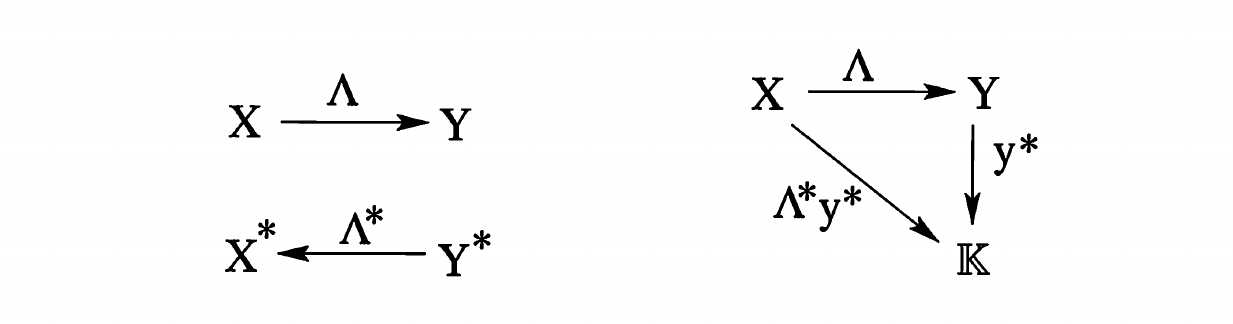
\includegraphics[width=0.75\linewidth]{adjoint.png}\\ \\
\begin{definition}[Orthogonal Space]
    
In the following, given a subset $V \subseteq X$, we define its orthogonal set as

\[
V^\perp = \{x^* \in X^* \mid \langle x^*, x\rangle  = 0 \text{ for all } x \in V\}.
\]

Similarly, if $W \subseteq X^*$, we define

\[
W^\perp = \{x \in X \mid \langle x^*, x\rangle  = 0 \text{ for all } x^* \in W\}.
\]
\end{definition}
\begin{theorem}[Properties of adjoint operators]
    Let X and Y be banach space and $A : X \to Y$ be a bounded linear operator, and let $A^* : Y^* \to X^*$ be its adjoint operator. Then:
\begin{itemize}
    \item[(i)] $\|A^*\| = \|A\|$.
    \item[(ii)] $\text{Ker}(A) = \text{Range}(A^*)^\perp$ and $\text{Ker}(A^*) = \text{Range}(A)^\perp$.
\end{itemize}
\end{theorem}
\begin{proof}
    Proof of (i): The statement (i) follows from:

    \[
    \|A\| = \sup \left\{ \|Ax\| : \|x\| \leq 1 \right\}
    = \sup \left\{ |\langle y^*, Ax\rangle | : \|x\| \leq 1, \|y^*\| \leq 1 \right\}
    \]
    
    \[
    = \sup \left\{ |\langle A^* y^*, x\rangle | : \|x\| \leq 1, \|y^*\| \leq 1 \right\}
    = \sup \left\{ \|A^* y^*\| : \|y^*\| \leq 1 \right\} 
    = \|A^*\|.
    \]
    
    Proof of (ii): To prove (ii), we observe that the following statements are all equivalent:
    
    \[
    x \in \text{Ker}(A),
    \]
    \[
    Ax = 0,
    \]
    \[
    \langle y^*, Ax\rangle  = 0 \quad \text{for all } y^* \in Y^*,
    \]
    \[
    \langle A^* y^*, x\rangle  = 0 \quad \text{for all } y^* \in Y^*,
    \]
    \[
    x \in \text{Range}(A^*)^\perp.
    \]
    
    Similarly, the following statements are all equivalent:
    
    \[
    y^* \in \text{Ker}(A^*),
    \]
    \[
    A^* y^* = 0,
    \]
    \[
    \langle A^* y^*, x\rangle  = 0 \quad \text{for all } x \in X,
    \]
    \[
    \langle y^*, Ax\rangle  = 0 \quad \text{for all } x \in X,
    \]
    \[
    y^* \in \text{Range}(A)^\perp.
    \]    
\end{proof}
\section{Reflexive spaces}
We consider a normed space $X$, it's dual space $X'$ and the dual space of $X' $, $X''$. $X''$. It is called the double dual or second dual of $X$.\\
Now we have a \textbf{Cannonical Mapping} $C: X \mapsto X''$ such that $$x \mapsto g_x$$ where $g_x(f) = f(x)$ for a fixed $x\in X $ and $f \in X'$. Thus in $X \subset X''$. 
\\ 
Now if C is a surjective map i.e. $\mathfrak{R} (C) = X''$ then We say that X is \textbf{Reflexive space}. Thus $C(X) = X''$.



\begin{lemma}
 For every fixed $x$ in a normed space $X$, the functional $g_x$ defined as above is a bounded linear functional on $X'$, so that $g_x \in X''$, and has the norm
\[
\|g_x\| = \|x\|.
\]
\end{lemma}
\begin{proof}
   Linearity of $g_x$ is known as follows:
   $$g_{ax+by}(f) = f(ax+by) = af(x) + bf(y)= ag_x(f) + bg_y(f)$$, 
\[
\|g_x\| = \sup_{f \in X', f \neq 0} \frac{|g_x(f)|}{\|f\|} = \sup_{f \in X', f \neq 0} \frac{|f(x)|}{\|f\|} = \|x\|.
\]
\end{proof}

\begin{lemma}[Cannonical mapping]
The canonical mapping $C$ given by (5) is an isomorphism of the normed space $X$ onto the normed space $\mathcal{R}(C)$, the range of $C$.

 
\end{lemma}
\begin{proof}
    Linearity of $C$ is seen as 
\[
g_{ax + \beta y}(f) = f(ax + \beta y) = \alpha f(x) + \beta f(y) = \alpha g_x(f) + \beta g_y(f).
\]

In particular, $ g_x - g_y  =  g_{x - y} $. Hence we obtain
\[
\|g_x - g_y\| = \|g_{x - y}\| = \|x - y\|.
\]

This shows that $C$ is isometric; it preserves the norm. Isometry implies injectivity. Also C is a surjective map from $X$ to $\mathcal{R}(C) $. Thus C is a bijection from $X$ to $\mathcal{R}(C) $. Hence it is a isomorphism.

\end{proof}

\begin{theorem}[completeness]
    If a normed space X is reflexive then it is complete hence banach space. 
    
\end{theorem}
\begin{proof}
    As $X''$ is a dual space of $X' $ hence it is complete being a bounded linear functional. and as X is reflexive hence $C(X) = X''$. Hence the completeness of $X$ follows from the completeness of $X''$ as $X$ is isomorphic to $X''$. 
\end{proof}
\section{Strong, Weak and Weak-Star Convergence}
\begin{definition}[Strong Convergence]
    A sequence $(x_n)$ in a normed space X is said to be strongly convergent if $\exists$ a x $\in X$ such that \[\lim_{n \to \infty} \| x_n - x \| = 0  \]
\end{definition}
\begin{definition}[Weak Convergence]
    A sequence $(x_n)$ in a normed space X is said to be weakly convergent if $\exists$ x $\in X $ such that for every $f \in X',$\[ \lim_{n \to \infty } f(x_n) = f(x)    \]

\end{definition}
\begin{lemma}[Weak convergence]
Let $(x_n)$ be a weakly convergent sequence in a normed space $X$, say, $x_n \rightharpoonup x$. Then:

\begin{enumerate}
\item The weak limit $x$ of $(x_n)$ is unique.
\item Every subsequence of $(x_n)$ converges weakly to $x$.
\item The sequence $(\|x_n\|)$ is bounded.
\end{enumerate}
\end{lemma}
\begin{proof}
\begin{enumerate}
\item Suppose that $x_n \rightharpoonup x$ as well as $x_n \rightharpoonup y$. Then $f(x_n) \to f(x)$ as well as $f(x_n) \to f(y)$. Since $(f(x_n))$ is a sequence of numbers, its limit is unique. Hence $f(x) = f(y)$, that is, for every $f \in X'$ we have

\[f(x) - f(y) = f(x - y) = 0.\]

This implies $x - y = 0$ and shows that the weak limit is unique.

\item $(2)$ follows from the fact that $(f(x_n))$ is a convergent sequence of numbers, so that every subsequence of $(f(x_n))$ converges and has the same limit as the sequence.
\item (c) Since $(f(x_n))$ is a convergent sequence of numbers,  $ \implies |f(x_n)| \leq c_f$ for all $n$, where $c_f$ is a constant depending on $f$ but not on $n$. Using the canonical mapping $C: X \to X''$ , we can define $g_n \in X''$ by

\[g_{x_n}(f) = f(x_n) \qquad \qquad f \in X'.\]

 Then for all $n$,

\[|g_{x_n}(f)| = |f(x_n)| \leq c_f,\]

that is, the sequence $(g_n(f))$ is bounded for every $f \in X'$. Since $X'$ is complete, the uniform boundedness theorem $ \implies (\|g_n\|)$ is bounded. Now $\|g_n\| = \|x_n\|$, so that (3) is proved.
\end{enumerate}
\end{proof}
\newpage
\begin{lemma}
Let $(x_n)$ be a sequence in Banach space $E$. Then:

\begin{itemize}
    \item[(i)] $[x_n \rightharpoonup x \text{ weakly in } \sigma(E, E^*)] \iff [\langle f, x_n \rangle \to \langle f, x \rangle \ \forall f \in E^*]$.
    
    \item[(ii)] If $x_n \to x$ strongly, then $x_n \rightharpoonup x$ weakly in $\sigma(E, E^*)$.
    
    \item[(iii)] If $x_n \rightharpoonup x$ weakly in $\sigma(E, E^*)$, then $(x_n)$ is bounded and $x \leq \liminf x_n$.
    
    \item[(iv)] If $x_n \rightharpoonup x$ weakly in $\sigma(E, E^*)$ and if $f_n \to f$ strongly in $E^*$ (i.e., $\|f_n - f\|_{E^*} \to 0$), then $\langle f_n, x_n \rangle \to \langle f, x \rangle$.
\end{itemize}

\end{lemma}
\begin{theorem}
 Let $E$ and $F$ be two Banach spaces and let $T$ be a linear operator from $E$ into $F$. Assume that $T$ is continuous in the strong topologies. Then $T$ is continuous from $E$ weak $\sigma(E, E^*)$ into $F$ weak $\sigma(F, F^*)$ and conversely.

\end{theorem}
\begin{definition}[Weak-Star Convergence]
    A sequence $(\phi_n)$ in a normed space $X^*$ Weak-Star Converges to $\phi \in X^*$ if \[ \lim_{n \to \infty} \phi_n (x) = \phi(x) \qquad \qquad \forall x \in X\]
\end{definition}
\begin{theorem}[Banach-Alaoglu]
    Let X be a seperable Banach space. Then every bounded sequence of linear functional in $X^*$ admits a Weak-Star Convergent Subsequence.
\end{theorem}
\section{Uniform Convexity }
\begin{definition}
 A Banach space $E$ is said to be uniformly convex if $\forall \, \epsilon > 0$, there exists $\delta > 0$ such that for any $x, y \in E$ with $\|x\| \leq 1$, $\|y\| \leq 1$, and $\|x - y\| > \epsilon$, it follows that

\[
\left\|\frac{x + y}{2}\right\| < 1 - \delta.
\]

\end{definition}
\begin{example}
 Let $E = \mathbb{R}^2$. The norm $\|x\|_2 = \sqrt{|x_1|^2 + |x_2|^2}$ is uniformly convex, while the norm $\|x\|_1 = |x_1| + |x_2|$ and the norm $\|x\|_\infty = \max(|x_1|, |x_2|)$ are not uniformly convex.

\end{example}

\begin{theorem}[Milman-Pettis]
    Every Convex Banach Space is Reflexive.
\end{theorem}
\section{Inner Product Spaces}
\begin{definition}
    Let \( H \) be a vector space. A inner product \( (u, v) \) is a bilinear form on \( H \times H \) with values in \( \mathbb{C} \) (i.e., a map from \( H \times H \) to \( \mathbb{C} \) that is linear in both variables) such that:
\begin{itemize}
    \item \textbf{Symmetry:} \( (u, v) = \overline{(v, u)} \) for all \( u, v \in H \),
    \item \textbf{Positive:} \( (u, u) \geq 0 \) for all \( u \in H \),
    \item \textbf{Definiteness:} \( (u, u) = 0 \Rightarrow u = 0 \).
\end{itemize}
\end{definition}

\setlength{\parskip}{1em}
\setlength{\parindent}{0em}
\renewcommand{\baselinestretch}{1.2}



\section{Definition and Basic Properties of Hilbert Spaces}

\textbf{Definition:} A \textbf{Hilbert space} \( H \) is a complete inner product space. 

\begin{itemize}
    \item It is a vector space equipped with an \textbf{inner product} \( \langle \cdot, \cdot \rangle \), which satisfies:
    \begin{enumerate}
        \item \(\langle x, y \rangle = \overline{\langle y, x \rangle}, \quad \forall x, y \in H\) (conjugate symmetry),
        \item \(\langle x, x \rangle \geq 0 \quad \text{and} \quad \langle x, x \rangle = 0 \iff x = 0\) (positive definiteness),
        \item \(\langle \alpha x + \beta y, z \rangle = \alpha \langle x, z \rangle + \beta \langle y, z \rangle, \quad \forall \alpha, \beta \in \mathbb{C}\) (linearity in the first argument).
    \end{enumerate}
    \item The inner product induces a norm:
    \[
    \|x\| = \sqrt{\langle x, x \rangle}, \quad x \in H.
    \]
    \item Completeness: Every Cauchy sequence \( (x_n) \subseteq H \) converges to a limit \( x \in H \), i.e., 
    \[
    \|x_n - x\| \to 0 \quad \text{as } n \to \infty.
    \]
\end{itemize}

\section{Orthogonality, Orthogonal Projections, and Hilbert Sums}

\subsection*{Orthogonality}
\begin{itemize}
    \item Two vectors \( x, y \in H \) are \textbf{orthogonal} if:
    \[
    \langle x, y \rangle = 0.
    \]
    \item For a subspace \( M \subseteq H \), the \textbf{orthogonal complement} \( M^\perp \) is:
    \[
    M^\perp = \{x \in H : \langle x, y \rangle = 0, \, \forall y \in M\}.
    \]
    \item \( H \) can be decomposed into the direct sum of \( M \) and \( M^\perp \):
    \[
    H = M \oplus M^\perp.
    \]
\end{itemize}

\subsection*{Orthogonal Projections}
\begin{itemize}
    \item Let \( M \) be a closed subspace of \( H \). For any \( x \in H \), there exists a unique decomposition:
    \[
    x = y + z, \quad y \in M, \, z \in M^\perp.
    \]
    \item The map \( P : H \to M \), defined by \( P(x) = y \), is called the \textbf{orthogonal projection} onto \( M \).
    \item Properties of \( P \):
    \begin{enumerate}
        \item \( P^2 = P \) (idempotence),
        \item \( P \) is a bounded linear operator: 
        \[
        \|P(x)\| \leq \|x\|, \quad \forall x \in H,
        \]
        \item \( P \) is self-adjoint:
        \[
        \langle P(x), y \rangle = \langle x, P(y) \rangle, \quad \forall x, y \in H,
        \]
        \item \( \ker(P) = M^\perp \quad \text{and} \quad \operatorname{im}(P) = M \),
        \item \( \langle P(x), z \rangle = 0, \, \forall z \in M^\perp \) (orthogonality of the projection).
    \end{enumerate}
\end{itemize}

\subsection*{Hilbert Sum of Subspaces}
\begin{itemize}
    \item Let \( M_1, M_2, \dots, M_n \) be subspaces of \( H \). The \textbf{Hilbert sum} is defined as:
    \[
    M_1 \oplus M_2 \oplus \cdots \oplus M_n = \left\{ x \in H : x = \sum_{i=1}^n x_i, \, x_i \in M_i, \, M_i \perp M_j \, \forall i \neq j \right\}.
    \]
    \item For an infinite family \( \{M_i\}_{i \in I} \) of pairwise orthogonal subspaces, the Hilbert sum is:
    \[
    \bigoplus_{i \in I} M_i = \left\{ x \in H : x = \sum_{i \in I} x_i, \, x_i \in M_i, \, \sum_{i \in I} \|x_i\|^2 < \infty \right\}.
    \]
    \item If \( H = \bigoplus_{i \in I} M_i \), then every \( x \in H \) can be uniquely expressed as:
    \[
    x = \sum_{i \in I} x_i, \quad x_i \in M_i.
    \]
\end{itemize}

\section{Orthonormal Bases and Parseval's Identity}
\begin{itemize}
    \item A set \( \{e_i\}_{i \in I} \subseteq H \) is \textbf{orthonormal} if:
    \[
    \langle e_i, e_j \rangle = 
    \begin{cases} 
    1 & \text{if } i = j, \\
    0 & \text{if } i \neq j.
    \end{cases}
    \]
    \item An orthonormal set \( \{e_i\} \) is a \textbf{basis} if:
    \[
    x = \sum_{i \in I} \langle x, e_i \rangle e_i, \quad \forall x \in H.
    \]
    (The series converges in the norm induced by the inner product.)
    \item Parseval's identity:
    \[
    \|x\|^2 = \sum_{i \in I} |\langle x, e_i \rangle|^2, \quad \forall x \in H.
    \]
\end{itemize}

\section{The Riesz Representation Theorem}
\textbf{Statement:} If \( H \) is a Hilbert space, then for every continuous linear functional \( f \in H^* \) (the dual space of \( H \)), there exists a unique \( y \in H \) such that:
\[
f(x) = \langle x, y \rangle, \quad \forall x \in H.
\]


















\end{document}
